\lab{Anisotropic Diffusion}{Anisotropic Diffusion}
\label{lab:AnisotropicDiffusion}

\objective{Demonstrate the use of finite difference schemes in image analysis.}
\labdependencies{FiniteDifferenceMethod,HeatFlow}

A common task in image processing is to remove extra static from an image.
This is most easily done by simply blurring the image, which can be accomplished by  treating the image as a rectangular domain and applying the diffusion (heat) equation:
\[u_t = c \Delta u\]
where $c$ is some diffusion constant and $\Delta$ is the Laplace operator.
Unfortunately, this also blurs the boundary lines between distinct elements of the image.

A more general form of the diffusion equation in two dimensions is:
\[u_t = \nabla\cdot \left( c(x,y,t) \nabla u \right)\]
where $c$ is a function representing the diffusion coefficient at each given point and time.
In this case, $\nabla \cdot$ is the divergence operator and $\nabla$ is the gradient.

To blur a picture uniformly, choose $c$ to be a constant function.
% , but we are often interested in \textit{preserving the edges} between features of the image.
Since $c$ controls how much diffusion is allowed at each point, it can be modified so that diffusion is minimized across edges in the image.
In this way we attempt to limit diffusion near the boundaries between different features of the image, and allow smaller details of the image (such as static) to blur away.
This method for image denoising is especially useful for denoising low quality images, and was first introduced by Pietro Perona and Jitendra Malik in 1987.
It is known as Anisotropic Diffusion or Perona-Malik Diffusion.

\section*{A Finite Difference Scheme}
Suppose we have some estimate $E$ of the rate of change at a given point in an image.
$E$ will be largest at the boundaries in the image.
We will then let $c(x,y,t) = g(E(x,y,t))$ where $g$ is some function such that $g(0)=1$ and $\displaystyle{\lim_{x \to \infty} g(x) = 0}$.
Thus $c$ will be small where $E$ is large, so that little diffusion occurs near the boundaries of different portions of the image.

We will model this system using a finite differencing scheme with an array of values at a 2D grid of points, and iterate through time.
Let $U_{l,m}^n$ be the discretized approximation of the function $u$, $n$ be the index in time, $l$ be the index along the $x$-axis, and $m$ be the index along the $y$-axis.

The Laplace operator can be approximated with the finite difference scheme
\[\Delta u = u_{xx}+u_{yy} \approx \frac{U_{l-1,m}^n - 2 U_{l,m}^n + U_{l+1,m}^n}{(\Delta x)^2} + \frac{U_{l,m-1}^n-2 U_{l,m}^n + U_{l,m+1}^n}{(\Delta y)^2}.\]
A good metric to use with images is to let the distance between each pixel be equal to one, so $\Delta x = \Delta y = 1$.
Rearranging terms, we obtain
\[\Delta u \approx (U_{l-1,m}^n - U_{l,m}^n) + (U_{l+1,m}^n - U_{l,m}^n) + (U_{l,m-1}^n - U_{l,m}^n) + (U_{l,m+1}^n - U_{l,m}^n).\]
Again, since we are working with images and not some time based problem, we can without loss of generality let $\Delta t = 1$, so we obtain the finite difference scheme
\[U_{l,m}^{n+1} = U_{l,m}^n + (U_{l-1,m}^n - U_{l,m}^n) + (U_{l+1,m}^n - U_{l,m}^n) + (U_{l,m-1}^n - U_{l,m}^n) + (U_{l,m+1}^n - U_{l,m}^n).\]
We will now limit the diffusion near the edges of objects by making the modification
\begin{equation}\label{eq:anisotropic}
\begin{aligned}
U_{l,m}^{n+1} = U_{l,m}^n + & \lambda \Big(g(|U_{l-1,m}^n - U_{l,m}^n|)(U_{l-1,m}^n - U_{l,m}^n) \\
			&+ g(|U_{l+1,m}^n - U_{l,m}^n|)(U_{l+1,m}^n - U_{l,m}^n) \\
			&+ g(|U_{l,m-1}^n - U_{l,m}^n|)(U_{l,m-1}^n - U_{l,m}^n) \\
			&+ g(|U_{l,m+1}^n - U_{l,m}^n|)(U_{l,m+1}^n - U_{l,m}^n)\Big),
\end{aligned}
\end{equation}
where $\lambda \leq \frac{1}{4}$ is the stability condition.

In this difference scheme, each term is affected most by nearby terms that are most similar to it, so less diffusion will happen anywhere there is a sharp difference between pixels.
This scheme also has the useful property that it does not increase or decrease the total brightness of the image.
Intuitively, this is because the effect of each point on its neighbors is exactly the opposite effect its neighbors have on it.

Two commonly used functions for $g$ are $g(x) = e^{-\left(\frac{x}{\sigma}\right)^2}$ and $g(x) = \frac{1}{1+\left(\frac{x}{\sigma}\right)^2}$.
The parameter $\sigma$ allows us to control how much diffusion decreases across boundaries, with larger $\sigma$ values allowing more diffusion.
Note that $g(0) = 1$ and $\displaystyle{\lim_{x\to \infty} g(x) = 0}$ for both functions.
In this lab we use $g(x)=e^{-\left(\frac{x}{\sigma}\right)^2}$.

It is worth noting that this particular difference scheme is \textit{not} an accurate finite difference scheme for the version of the diffusion equation we discussed before, but it \textit{does} accomplish the same thing in the same way.
As it turns out, this particular scheme is the solution to a slightly different diffusion PDE, but can still be used the same way.

For this lab's examples we read in the image using the \li{imageio.imread} function, and normalized it so that the colors are represented as floating point values between 0 and 1.
An image can converted to black and white when it is read by including the argument \li{as_gray=True}.

\begin{lstlisting}
from matplotlib import cm, pyplot as plt
from imageio import imread

# To read in an image, convert it to grayscale, and rescale it.
picture = imread('balloon.jpg', as_gray=True) * 1./255

# To display the picture as grayscale
plt.imshow(picture, cmap=cm.gray)
plt.show()
\end{lstlisting}

\subsection*{Simplifying Calculations}\label{sec:simp}

You will notice that the algorithm given in \ref{eq:anisotropic} does not describe what to do for the edges and corners of $U^{n+1}$.
In these cases we will simply eliminate the undefined terms in the algorithm.
For example, the top edge equation becomes
\begin{align*}
U_{l,m}^{n+1} = U_{l,m}^n + & \lambda (g(|U_{l+1,m}^n - U_{l,m}^n|)(U_{l+1,m}^n - U_{l,m}^n) \\
                    & + g(|U_{l,m+1}^n - U_{l,m}^n|)(U_{l,m+1}^n - U_{l,m}^n)) \\
					& + g(|U_{l,m-1}^n - U_{l,m}^n|)(U_{l,m-1}^n - U_{l,m}^n)),
\end{align*}
and top left corner equation becomes
\begin{align*}
U_{l,m}^{n+1} = U_{l,m}^n + & \lambda (g(|U_{l+1,m}^n - U_{l,m}^n|)(U_{l+1,m}^n - U_{l,m}^n) \\
					& + g(|U_{l,m+1}^n - U_{l,m}^n|)(U_{l,m+1}^n - U_{l,m}^n)).
\end{align*}
Essentially we are only using the terms of the difference scheme that are actually defined.

To help facilitate this we can create a larger "padded" matrix that will make these calculations easy to do.
This padded matrix will have an extra row on the top and bottom, and an extra column on either side of the original matrix.
These extra rows and columns will duplicate the outer edge of the original matrix.

So if our original array \li{X} has shape \li{m,n}, then our padded array \li{Y} has shape \li{m+2,n+2}.
The top edge of \li{Y} will be defined so that \li{Y[0,1:-1] == X[0,:]} is true, and the rest of the edges of \li{Y} follow the same pattern.

Notice that this allows us to simply implement the algorithm found in \ref{eq:anisotropic} without having to make special cases for the edges and corners, since those previously undefined terms become zero when using the padded matrix.

\begin{problem}
\label{prob:anisdiff_bw}
Complete the following function, by implementing the anisotropic diffusion algorithm found in \ref{eq:anisotropic} for black and white images.
Use the padded array technique found in the Simplifying Calculations section.


In your function, use
\[g(x) = e^{-\left(\frac{x}{\sigma}\right)^2}\]

\begin{lstlisting}
def anisdiff_bw(U, N, lambda_, g):
    """ Run the Anisotropic Diffusion differencing scheme
    on the array U of grayscale values for an image.
    Perform N iterations, use the function g
    to limit diffusion across boundaries in the image.
    Operate on U inplace to optimize performance. """
    pass
\end{lstlisting}
Run the function on \li{balloon.jpg}.
Show the original image and the diffused image for $\sigma = .1$, $\lambda = .25$, $N = 5, 20, 100$.
\end{problem}

\newpage
\vfill
\begin{figure}[ht]
\begin{minipage}[b]{0.45\linewidth}
\centering
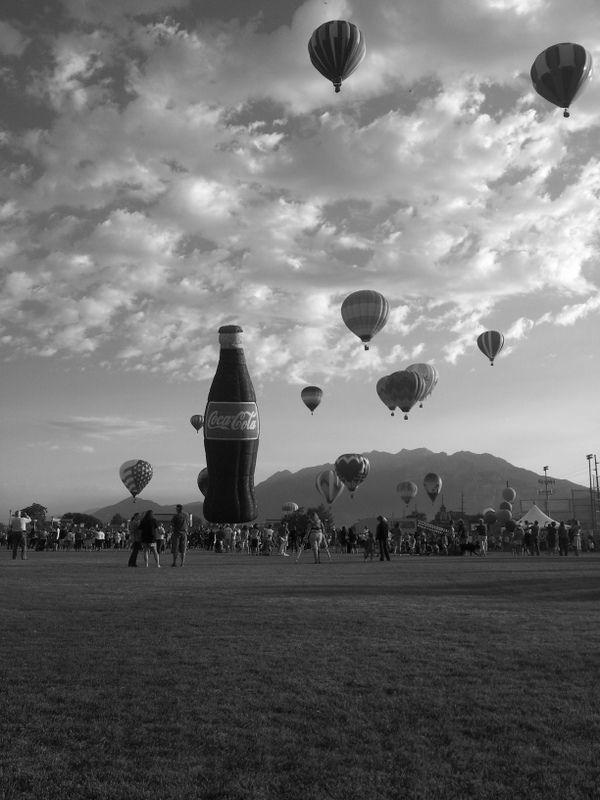
\includegraphics[width=\textwidth]{figures/balloon_grayscale.jpg}
\caption*{original image}
\end{minipage}
\hspace{0.5cm}
\begin{minipage}[b]{0.45\linewidth}
\centering
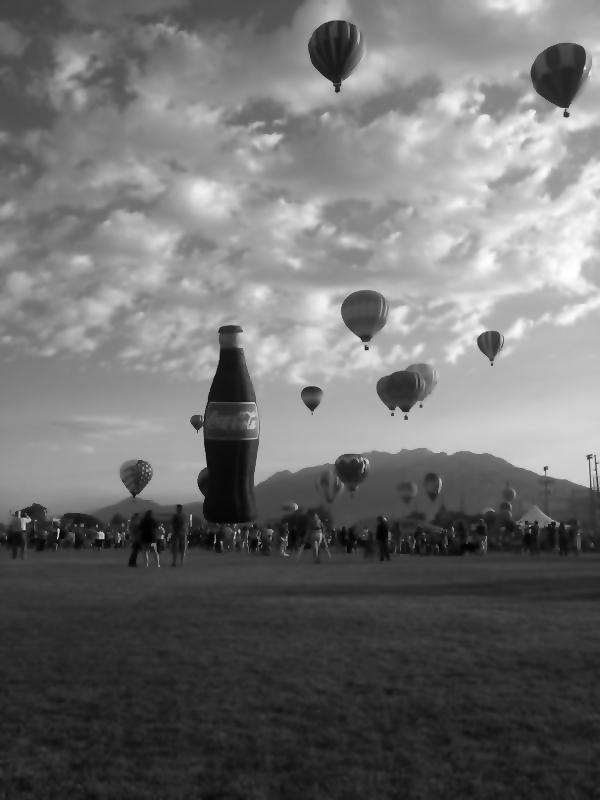
\includegraphics[width=\textwidth]{figures/balloon_grayscale_5.jpg}
\caption*{5 iterations with $\sigma = .1$ and $\lambda = .25$}
\end{minipage}
\begin{minipage}[b]{0.45\linewidth}
\centering
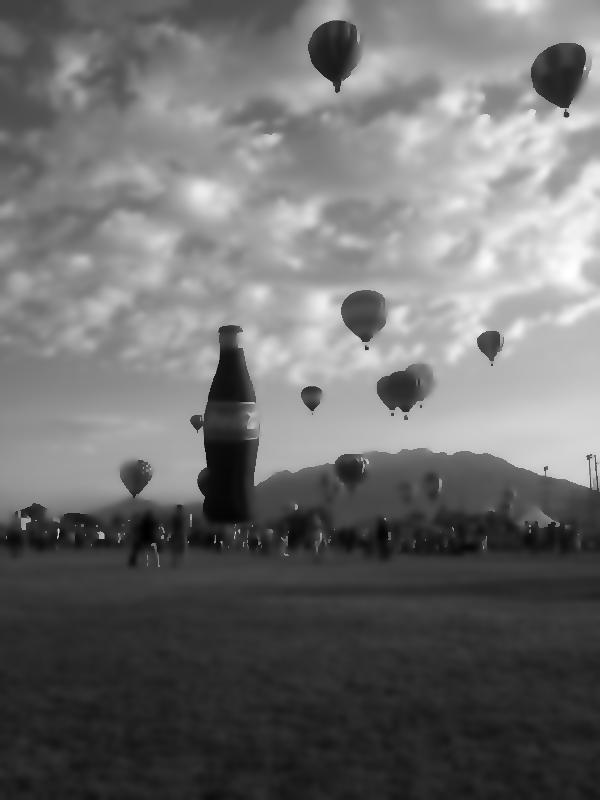
\includegraphics[width=\textwidth]{figures/balloon_grayscale_20.jpg}
\caption*{20 iterations}
\end{minipage}
\hspace{0.5cm}
\begin{minipage}[b]{0.45\linewidth}
\centering
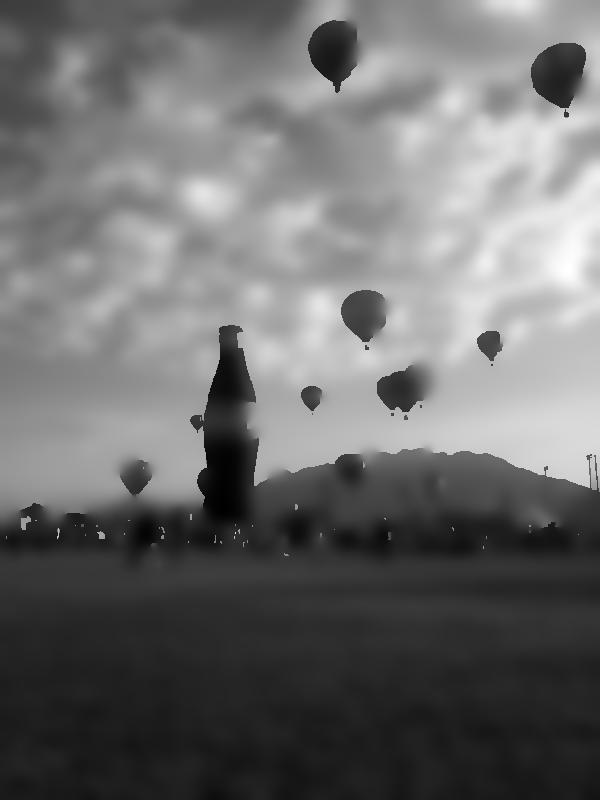
\includegraphics[width=\textwidth]{figures/balloon_grayscale_100.jpg}
\caption*{100 iterations}
\end{minipage}
\end{figure}
\vfill
\clearpage

\section*{Color Schemes}

Colored images can be processed in a similar manner.
Instead of being represented as a two-dimensional array, colored images are represented as three dimensional arrays.
The third dimension is used to store the intensities of each of the standard 3 colors.
This diffusion process can be carried out in the exact same way, on each of the arrays of intensities for each color, but instead of detecting edges just in one color, we need to detect edges in any color, so instead of using something of the form $g(|U_{l+1,m}^n - U_{l,m}^n|)$ as before, we will now use something of the form $g(||U_{l+1,m}^n - U_{l,m}^n||)$, where $U_{l+1,m}^n$ and $U_{l,m}^n$ are vectors now instead of scalars.
The difference scheme can be treated as an equation on vectors in 3-space and now reads:
\begin{align*}
U_{l,m}^{n+1} = U_{l,m}^n + & \lambda (g(||U_{l-1,m}^n - U_{l,m}^n||)(U_{l-1,m}^n - U_{l,m}^n) \\
					& + g(||U_{l+1,m}^n - U_{l,m}^n||)(U_{l+1,m}^n - U_{l,m}^n) \\
					& + g(||U_{l,m-1}^n - U_{l,m}^n||)(U_{l,m-1}^n - U_{l,m}^n) \\
					& + g(||U_{l,m+1}^n - U_{l,m}^n||)(U_{l,m+1}^n - U_{l,m}^n))
\end{align*}

When implementing this scheme for colored images, use the $2$-norm on 3-space, i.e $||x||=\sqrt{x_1^2+x_2^2+x_3^2}$ where $x_1$, $x_2$, and $x_3$ are the different coordinates of $x$.

\begin{problem}
Complete the following function to process a colored image.
You may modify your code from the previous problem.
Measure the difference between pixels using the $2$-norm.
Use the corresponding vector versions of the boundary conditions given in Problem \ref{prob:anisdiff_bw}.

\begin{lstlisting}
def anisdiff_color(U, N, lambda_, g):
    """ Run the Anisotropic Diffusion differencing scheme
    on the array U of color values for an image.
    Perform N iterations, use the function g = e^{-x^2/sigma^2}
    to limit diffusion across boundaries in the image.
    Operate on U inplace to optimize performance. """
    pass
\end{lstlisting}
Run the function on \li{balloons_color.jpg}.
Show the original image and the diffused image for $\sigma = .1$, $\lambda = .25$, $N = 5, 20, 100$.

Hint: If you have an $m \times n \times 3$ matrix representing the RGB differences of each pixel, then to find a matrix representing the norm of the differences, you can use the following code.
This code squares each value and sums along the last axis, and takes the square root.
In order to keep the dimension size of the matrix and aid in broadcasting, you must use \li{keepdims=True}.

\begin{lstlisting}
# x is mxnx3 matrix of pixel color values
norm = np.sqrt(np.sum(x**2, axis=2, keepdims=True))
\end{lstlisting}

\end{problem}

\newpage
\section*{Noisy Images}

\begin{problem}
Use the following code to add noise to your grayscale image.

\begin{lstlisting}
from numpy.random import randint

image = imread('balloon.jpg', as_gray=True)
x, y = image.shape
for i in range(x*y//100):
	image[randint(x),randint(y)] = 127 + randint(127)
\end{lstlisting}

Run \li{anisdiff_bw()} on the noisy image with $\sigma=.1$, $\lambda=.25$, $N=20$.
Display the original image and the noisy image.
Explain why anisotropic diffusion does not smooth out the noise.

Hint: Don't forget to rescale.
\end{problem}


\section*{Minimum Bias}

This sort of anisotropic diffusion can be very effective, but, depending on the image, it may also smear out edges that do not have large differences between them.
An example of this limitation can be seen in Figure \ref{fig:anisdif_smearing}

\begin{figure}
\begin{minipage}[b]{.45\linewidth}
\centering
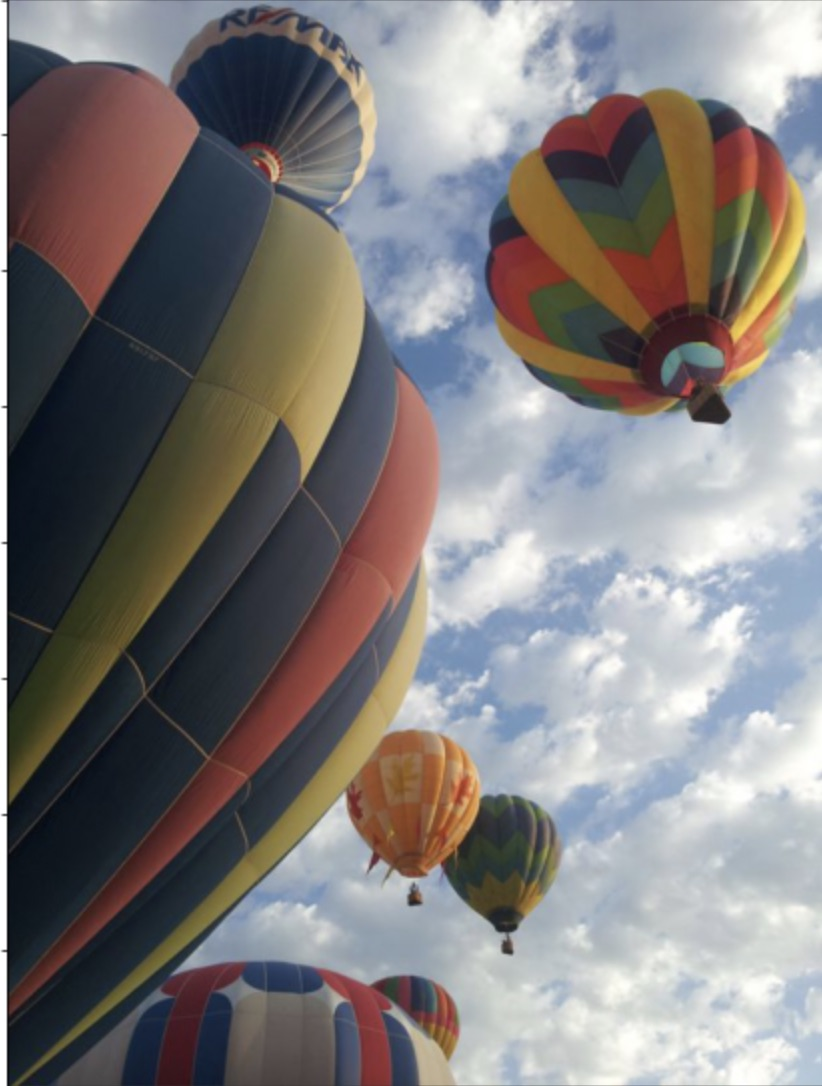
\includegraphics[width=\textwidth]{figures/original_color_img_prob2.jpg}
\caption*{original image}
\end{minipage}
\hspace{0.5cm}
\begin{minipage}[b]{0.45\linewidth}
\centering
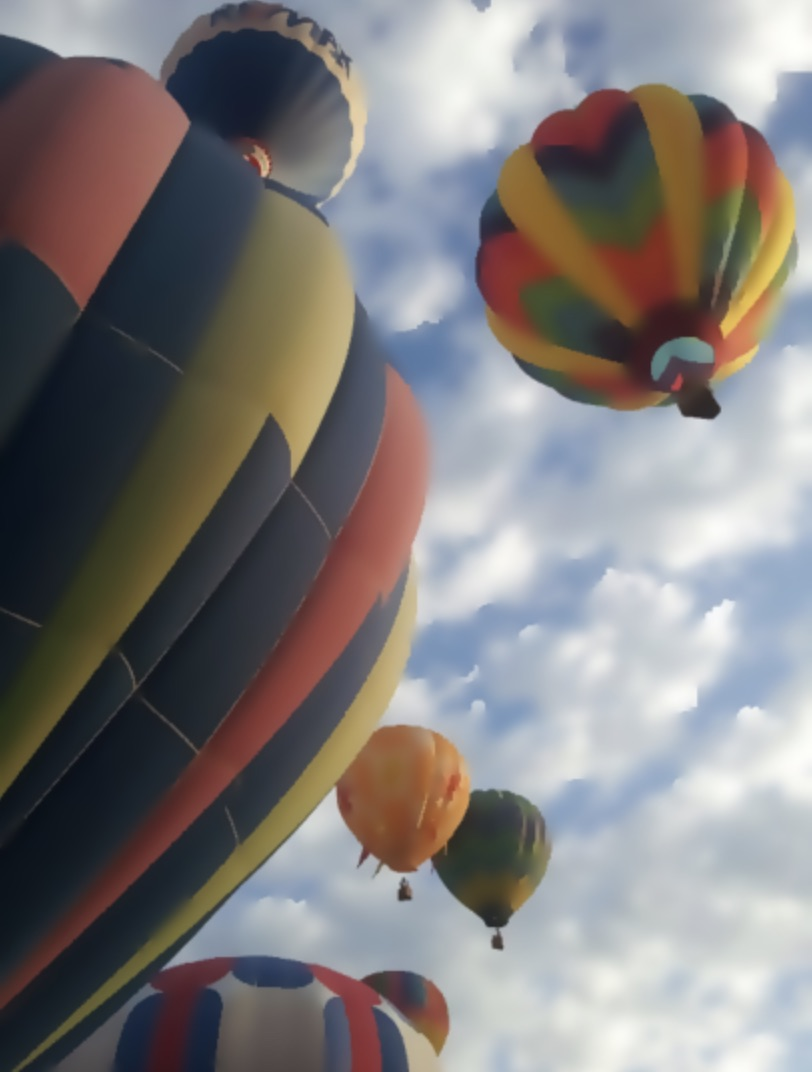
\includegraphics[width=\textwidth]{figures/50_iterations_color_prob2.jpg}
\caption*{after 50 iterations}
\end{minipage}
\caption{Smearing of similar colors when using an anisotropic diffusion filter.}
\label{fig:anisdif_smearing}
\end{figure}

As we can see, after 100 iterations, some of the boundaries between similar shades of grey have smeared unevenly. You may still have to look closely to see it.
This can be counteracted somewhat by further decreasing the $\sigma$ value, but if we have random noise throughout the image, this will not remove it.
If we have random static in the image, we can remove this using a modified version of the filter.
Instead of measuring the rate of change in the picture in each direction, we change each point according to whether or not any of its adjacent points have roughly the same value it has.
This is called a minimum-biased filter.
This sort of trick is especially good for removing isolated pixels that are different from those around them.
A very simple way to do this is by taking the average of the two smallest differences between each pixel and its eight neighbors and using that in place of $g$ in the difference scheme above.
Along the boundaries, we do not have 8 neighbors for each pixel, but we can get by by just using the pixels we have and eliminating the other terms in the difference scheme, just as we did before.
This will make it so that points that neighbor points of similar value will not be changed, while points that do not match their surroundings will be faded to become more like the points surrounding them.
This does not have the same symmetrical diffusion as the other scheme, i.e. if one pixel changes, it does not necessarily change its neighboring pixels by the same amount.
As long as you leave $\lambda \leq \frac{1}{4}$ and you have scaled the pixels to have floating point values between 0 and 1, the scheme will still remain within its minimum and maximum bounds, since the tendency is always to move points closer to the values of their neighbors.
To demonstrate the action of such a filter, we make changes to random pixels in the color version of the same photo and use both filters to remove the noise we have added.
Below, we include an example where we have added noise to the color version of that same picture, then used a minimum-biased filter to diminish the noise and the original filter to smooth what remains.

\begin{problem}

Implement the minimum-biased finite difference scheme described above.
Add noise to \li{balloons_color.jpg} using the provided code below, and clean it using your implementation.
Show the original image, the noised image, and the cleaned image.

\begin{lstlisting}
image = imread('balloons_color.jpg')
x,y,z = image.shape
for dim in range(z):
    for i in range(x*y//100):
        # Assign a random value to a random place
        image[randint(x),randint(y),dim] = 127 + randint(127)
\end{lstlisting}
Hint: Don't forget to rescale.

\end{problem}

\newpage
\vfill
\begin{figure}[ht]
\begin{minipage}[b]{0.45\linewidth}
\centering
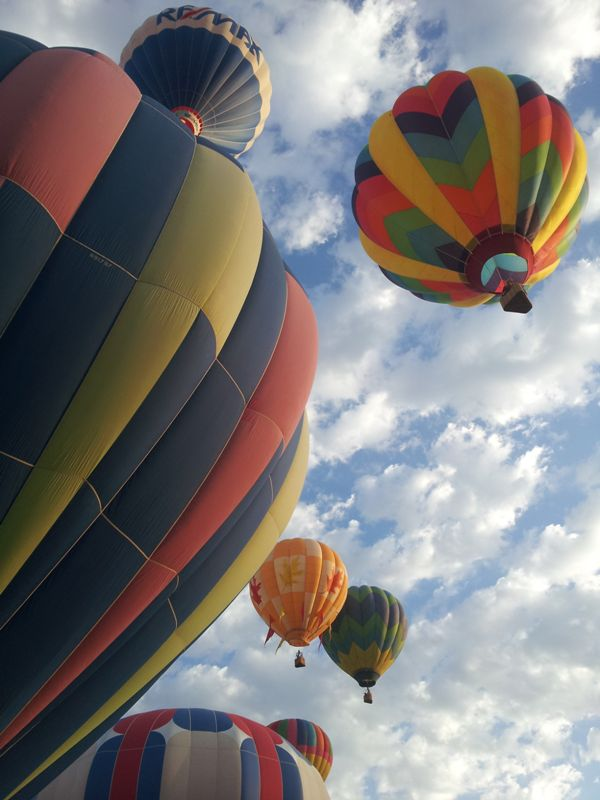
\includegraphics[width=\textwidth]{figures/baloons_resized_color.jpg}
\caption*{original image}
\end{minipage}
\hspace{0.5cm}
\begin{minipage}[b]{0.45\linewidth}
\centering
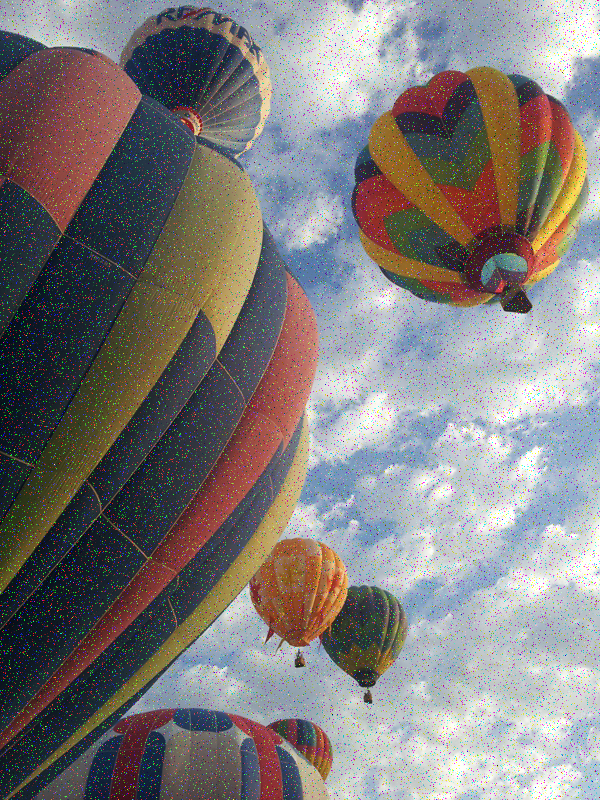
\includegraphics[width=\textwidth]{figures/baloons_resized_noisy.png}
\caption*{randomly changed 100000 color values}
\end{minipage}
\begin{minipage}[b]{0.45\linewidth}
\centering
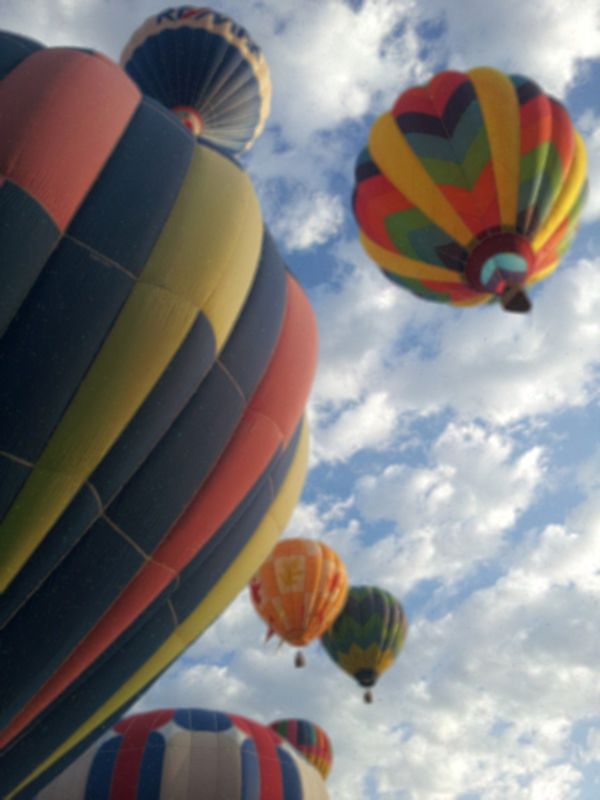
\includegraphics[width=\textwidth]{figures/baloons_resized_minbias.jpg}
\caption*{300 iterations of a min-biased scheme}
\end{minipage}
\hspace{0.5cm}
\begin{minipage}[b]{0.45\linewidth}
\centering
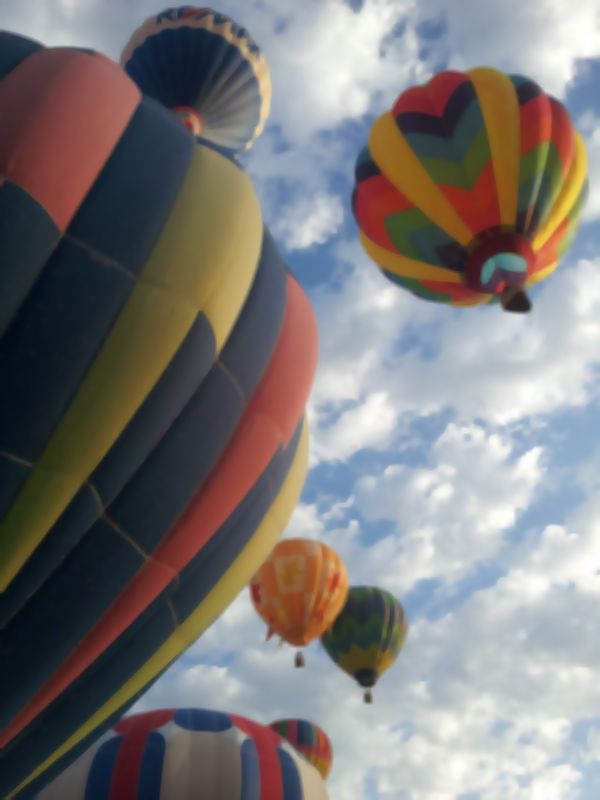
\includegraphics[width=\textwidth]{figures/baloons_resized_both.jpg}
\caption*{after 8 additional iterations of the first filter with $\lambda=.25$ and $\sigma=.04$.}
\end{minipage}
\end{figure}
\vfill
\clearpage

\nocite{Perona1988,Kim2009}
